\chapter{Background}
\label[chapter]{chapter:background}

...

\section{Coordinate Systems}
\label{sec:coordinate_systems}

\begin{center}
    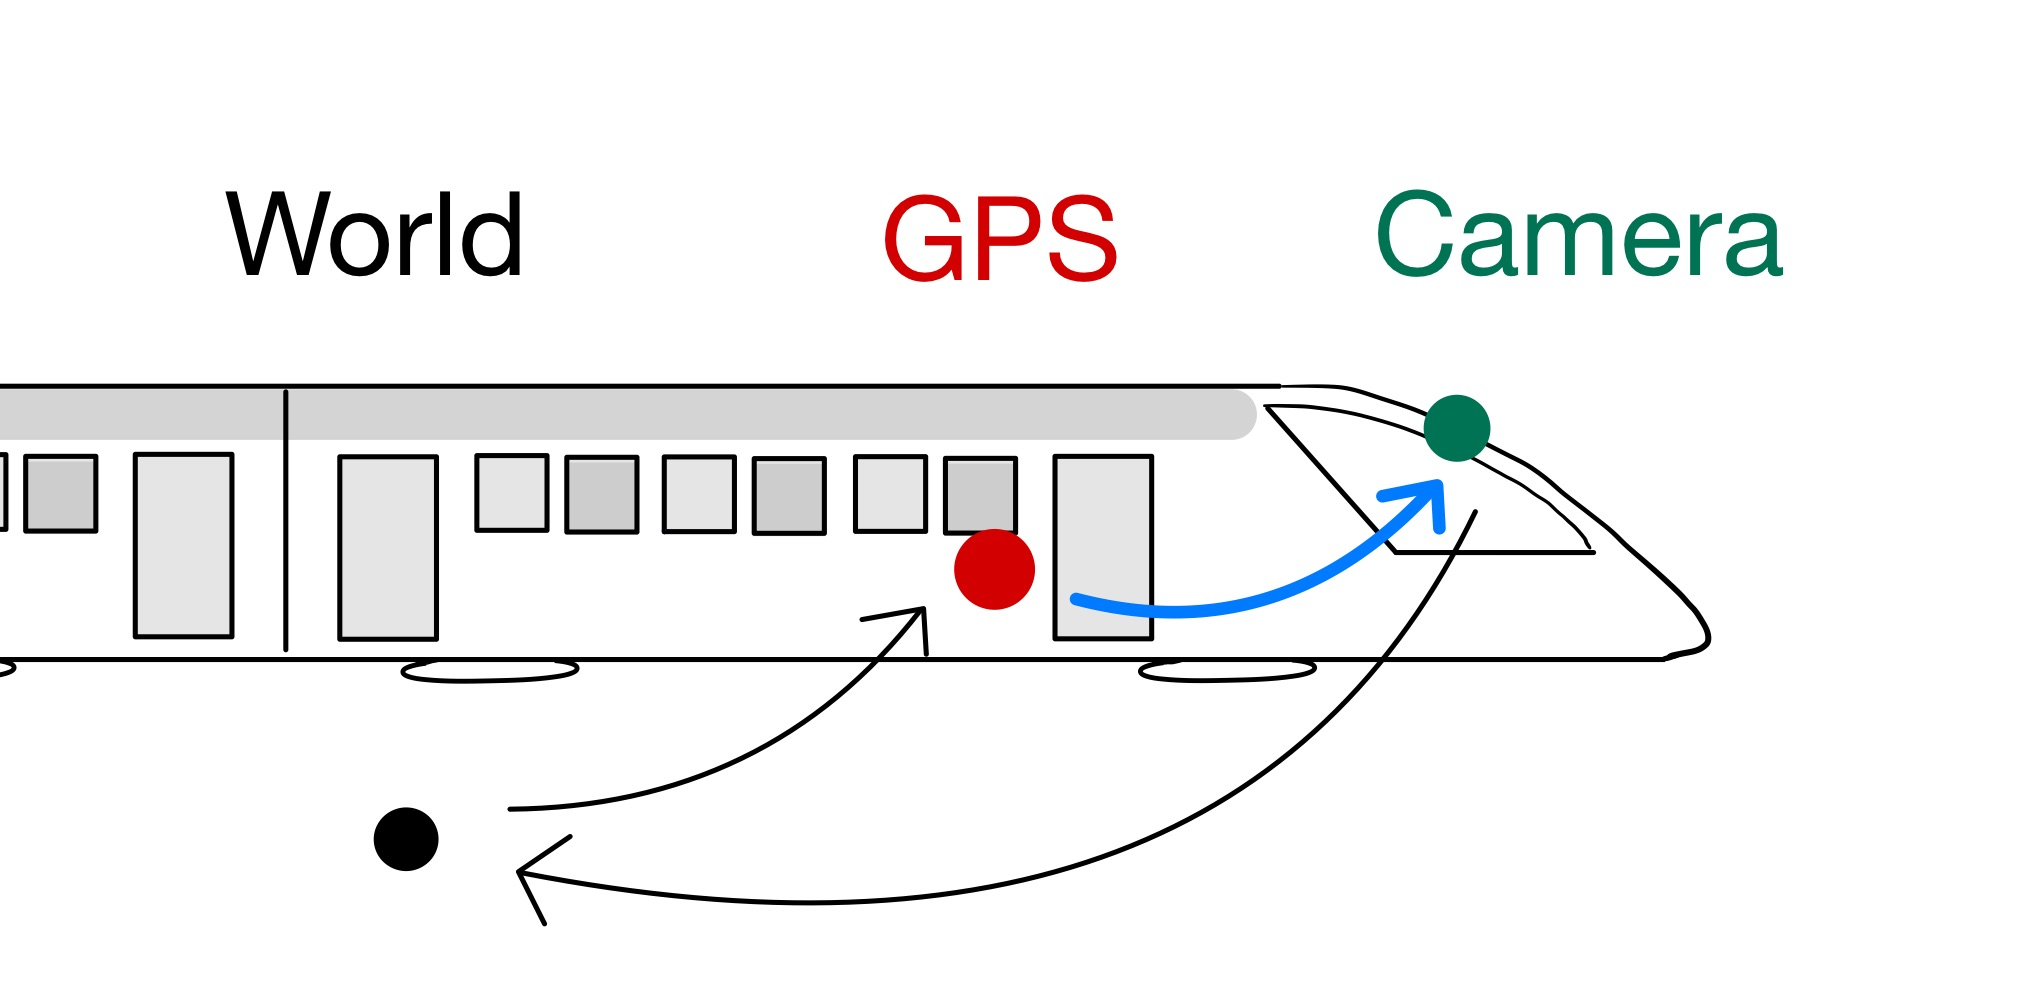
\includegraphics[width=0.5\textwidth]{images/coordinate_systems}
\end{center}

World: UTM coordinates \\

GPS \\

Camera frame \\

% how to scale table to make rows less dense?

\renewcommand{\arraystretch}{1.2}

\begin{table}
\begin{center}
    \caption{Descriptive directions and rotations, with associated GPS and camera axes.}
    \begin{tabular}{ |l|l|c|c| }
        \hline
        \textbf{Direction} & \textbf{Rotation} & \textbf{GPS axis} & \textbf{Camera axis} \\ 
        \hline
        Longitudinal (forward) & Roll & $+X_{GPS}$ & $+Z_{cam}$ \\ 
        Lateral (sideways, right) & Pitch & $+Y_{GPS}$ & $+X_{cam}$ \\ 
        Vertical (upwards) & Yaw & $+Z_{GPS}$ & $-Y_{cam}$ \\
        \hline
    \end{tabular}
\end{center}
\end{table}

Actual camera frame will change, depending on the orientation of the camera. This is an initial approximation.

\section{Coordinate Transformations}
\label{sec:coordinate_transformations}

In order to efficiently transform points between the different coordinate systems, namely those described in the previous section, it is important to understand the underlying methods. This section summarizes the most important concepts.

For the purpose of this project, homogeneous transformation matrices have been used most of the time since they are more intuitive. However, quaternions are used for the optimization, where they are dynamically adapted, since they are not prone to numerical singularities.

\subsection{Homogeneous Transformation Matrix}

Transformation, including both translation and rotation, of a vector to point $P$, from initial frame $\mathcal A$ to frame $\mathcal B$. This is achieved using the rotation matrix $R_{\mathcal B \mathcal A}$ (notation: frame $\mathcal A$ to frame $\mathcal B$) and translation vector $_\mathcal B \vec t_{BA}$ (notation: from point $A$ to point $B$, expressed in frame $\mathcal B$). To avoid computation issues, it is crucial to remember which frames the vectors are expressed in.
\begin{equation}
    \label[equation]{eq:homogeneous_transformation}
    _\mathcal B \vec r_{BP} = _\mathcal B \vec t_{BA} + R_{\mathcal B \mathcal A} \cdot _\mathcal A \vec r_{AP}
\end{equation}

% \begin{equation}
%     \label[equation]{eq:homogeneous_transformation_reversed}
%     _\mathcal A \vec r_{AP} = _\mathcal A \vec t_{AB} + R_{\mathcal A \mathcal B} \cdot _\mathcal B \vec r_{BP}
% \end{equation}

This can also be combined as a homogeneous transformation matrix $H_{\mathcal B \mathcal A}$.

\begin{equation}
    \label[equation]{eq:homogeneous_transformation_matrix}
    \begin{bmatrix} _\mathcal B \vec r_{BP} \\ 1 \end{bmatrix} = \underbrace{\begin{bmatrix} R_{\mathcal B \mathcal A} & _\mathcal B \vec t_{BA} \\ \vec 0_{1\times 3} & 1 \end{bmatrix}}_{H_{\mathcal B \mathcal A}} \cdot \begin{bmatrix} _\mathcal A \vec r_{AP} \\ 1 \end{bmatrix}
\end{equation}

% \begin{equation}
%     \label[equation]{eq:homogeneous_transformation_matrix_reversed}
%     \begin{bmatrix} _\mathcal A \vec r_{AP} \\ 1 \end{bmatrix} = \underbrace{\begin{bmatrix} R_{\mathcal A \mathcal B} & _\mathcal A \vec t_{AB} \\ \vec 0_{1\times 3} & 1 \end{bmatrix}}_{H_{\mathcal A \mathcal B}} \cdot \begin{bmatrix} _\mathcal B \vec r_{BP} \\ 1 \end{bmatrix}
% \end{equation}

To determine the inverse of a homogeneous transformation matrix, the translation vector need not only be reversed but also rotated to the new frame, while the rotation matrix is simply transposed.

\begin{equation}
    \label[equation]{eq:homogeneous_transformation_matrix_inverse}
    H_{\mathcal A \mathcal B} = \begin{bmatrix} R_{\mathcal A \mathcal B} & _\mathcal A \vec t_{AB} \\ \vec 0_{1\times 3} & 1 \end{bmatrix}
    = \begin{bmatrix} R_{\mathcal B \mathcal A}^T & -R_{\mathcal B \mathcal A}^T \cdot _\mathcal B \vec t_{BA} \\ \vec 0_{1\times 3} & 1 \end{bmatrix} 
\end{equation}

\subsection{Quaternion Rotation}

Definition of a quaternion $\vec q$ (4D vector) and its conjugate $\vec q^*$.

\begin{equation}
    \label[equation]{eq:quaternion_definition}
    \vec q = q_w + q_x\cdot \vec i + q_y\cdot \vec j + q_z\cdot \vec k = \begin{bmatrix} q_w \\ q_x \\ q_y \\ q_z \end{bmatrix} \qquad
    \vec q^* = \begin{bmatrix} q_w \\ -q_x \\ -q_y \\ -q_z \end{bmatrix}
\end{equation}

Must be a unit quaternion (scaled to unit norm)

Rotation using the quaternion product $\otimes$ (equal to cross-product minus dot-product)

\begin{equation}
    \label[equation]{eq:quaternion_rotation}
    \begin{bmatrix} 0 \\ _\mathcal B \vec r \end{bmatrix} = \vec q_{\mathcal B \mathcal A} \otimes \begin{bmatrix} 0 \\ _\mathcal A \vec r \end{bmatrix} \otimes \vec q_{\mathcal B \mathcal A}^*
\end{equation}

\section{Camera Reprojection \& Image Undistortion}

\subsection{Reprojection via the Pinhole Camera Model}

Reprojection of coordinates $(x,y,z)$ in the camera frame to pixel coordinates $(u,v)$ in the image plane. The variables $f_x$ and $f_y$ are the focal lengths in pixels, while $c_x$ and $c_y$ are the principal point coordinates in pixels.
\begin{align}
    \label[equation]{eq:camera_projection}
    u &= f_x \cdot \Big(\frac{x}{z}\Big) + c_x \\
    v &= f_y \cdot \Big(\frac{y}{z}\Big) + c_y
\end{align}

This can also be written in matrix form, with the camera instrinsics matrix $K$, where the variable $\lambda$ is the depth scaling factor since infinitely many 3D points would project to the same 2D point.

\begin{equation}
    \label[equation]{eq:camera_projection_matrix}
    \lambda \begin{bmatrix} u \\ v \\ 1 \end{bmatrix} = \underbrace{\begin{bmatrix} f_x & 0 & c_x\\ 0 & f_y & c_y \\ 0 & 0 & 1 \end{bmatrix}}_K \cdot \begin{bmatrix} x \\ y \\ z \end{bmatrix}
\end{equation}


\subsection{Image Undistortion: Equidistant Model}
\label{sec:undistortion}

\begin{align}
    r &= \sqrt{u^2 + v^2} \\
    \theta &= \arctan(r)
\end{align}

\begin{equation}
    \theta_d = \theta (1+ k_1\cdot\theta^2 + k_2\cdot\theta^4 + k_3\cdot\theta^6 + k_4\cdot\theta^8)
\end{equation}

...

Done using OpenCV fisheye

\section{Iterative Closest Points (ICP)}
\label{sec:iterative_closest_points}

Optimization
